\subsection{Multiplication factor dynamics}

\begin{frame}
\frametitle{Multiplication factor dynamics after shutdown}
\begin{textblock*}{12.5cm}(0.2cm,1.5cm) % {block width} (coords)
\begin{columns}
	\column[t]{6cm}
	\begin{figure}[t]
		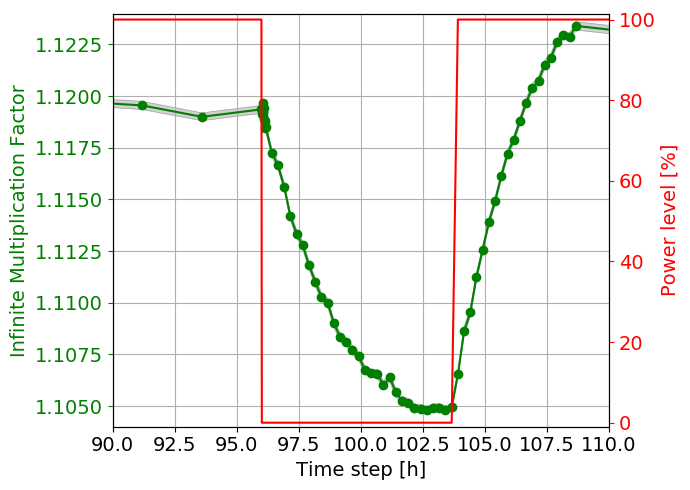
\includegraphics[width=\linewidth]{./images/pwr_keff_zoomed.png}
		\vspace{-6mm}
		\caption{Multiplication factor for PWR assembly after 
		shutdown ($\sigma\pm20$pcm shaded).}
	\end{figure}
		\vspace{-5mm}
	\begin{enumerate}             
		\item $-1500pcm$ reactivity insertion due to $^{135}$Xe poisoning
		\item $k_{\infty}$ reached local minima $\approx7$ hrs after shutdown
		\item overall reactivity swing $1750pcm$
	\end{enumerate}

	\column[t]{6cm}
	\visible<2->{

		\begin{figure}[t]
		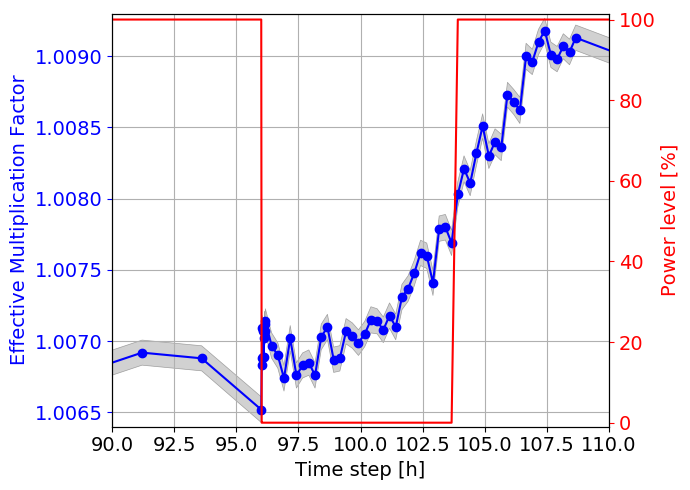
\includegraphics[width=\linewidth]{./images/tap_keff_zoomed.png}
		\vspace{-6mm}
		\caption{Multiplication factor for
TAP after 
			shutdown ($\sigma\pm7.5$pcm shaded).}
		\end{figure}
		\vspace{-5mm}
		\begin{enumerate}             
		\item $+130pcm$ reactivity insertion because loss of $^{135}$Xe from  
		decaying to $^{135}$Cs is larger than gain from $^{135}$I decay
		\item $k_{\infty}$ has no local minima
		\item overall reactivity swing $270pcm$
		\end{enumerate}

	}

\end{columns}
\end{textblock*}
\end{frame}

\subsection{$^{135}$Xe/$^{135}$I balance}
\begin{frame}
\frametitle{Fuel salt composition dynamics}
\begin{textblock*}{12.5cm}(0.2cm,2cm) % {block width} (coords)
	\begin{columns}[t,onlytextwidth]
		\column{.5\textwidth}
		\begin{figure}[t]
	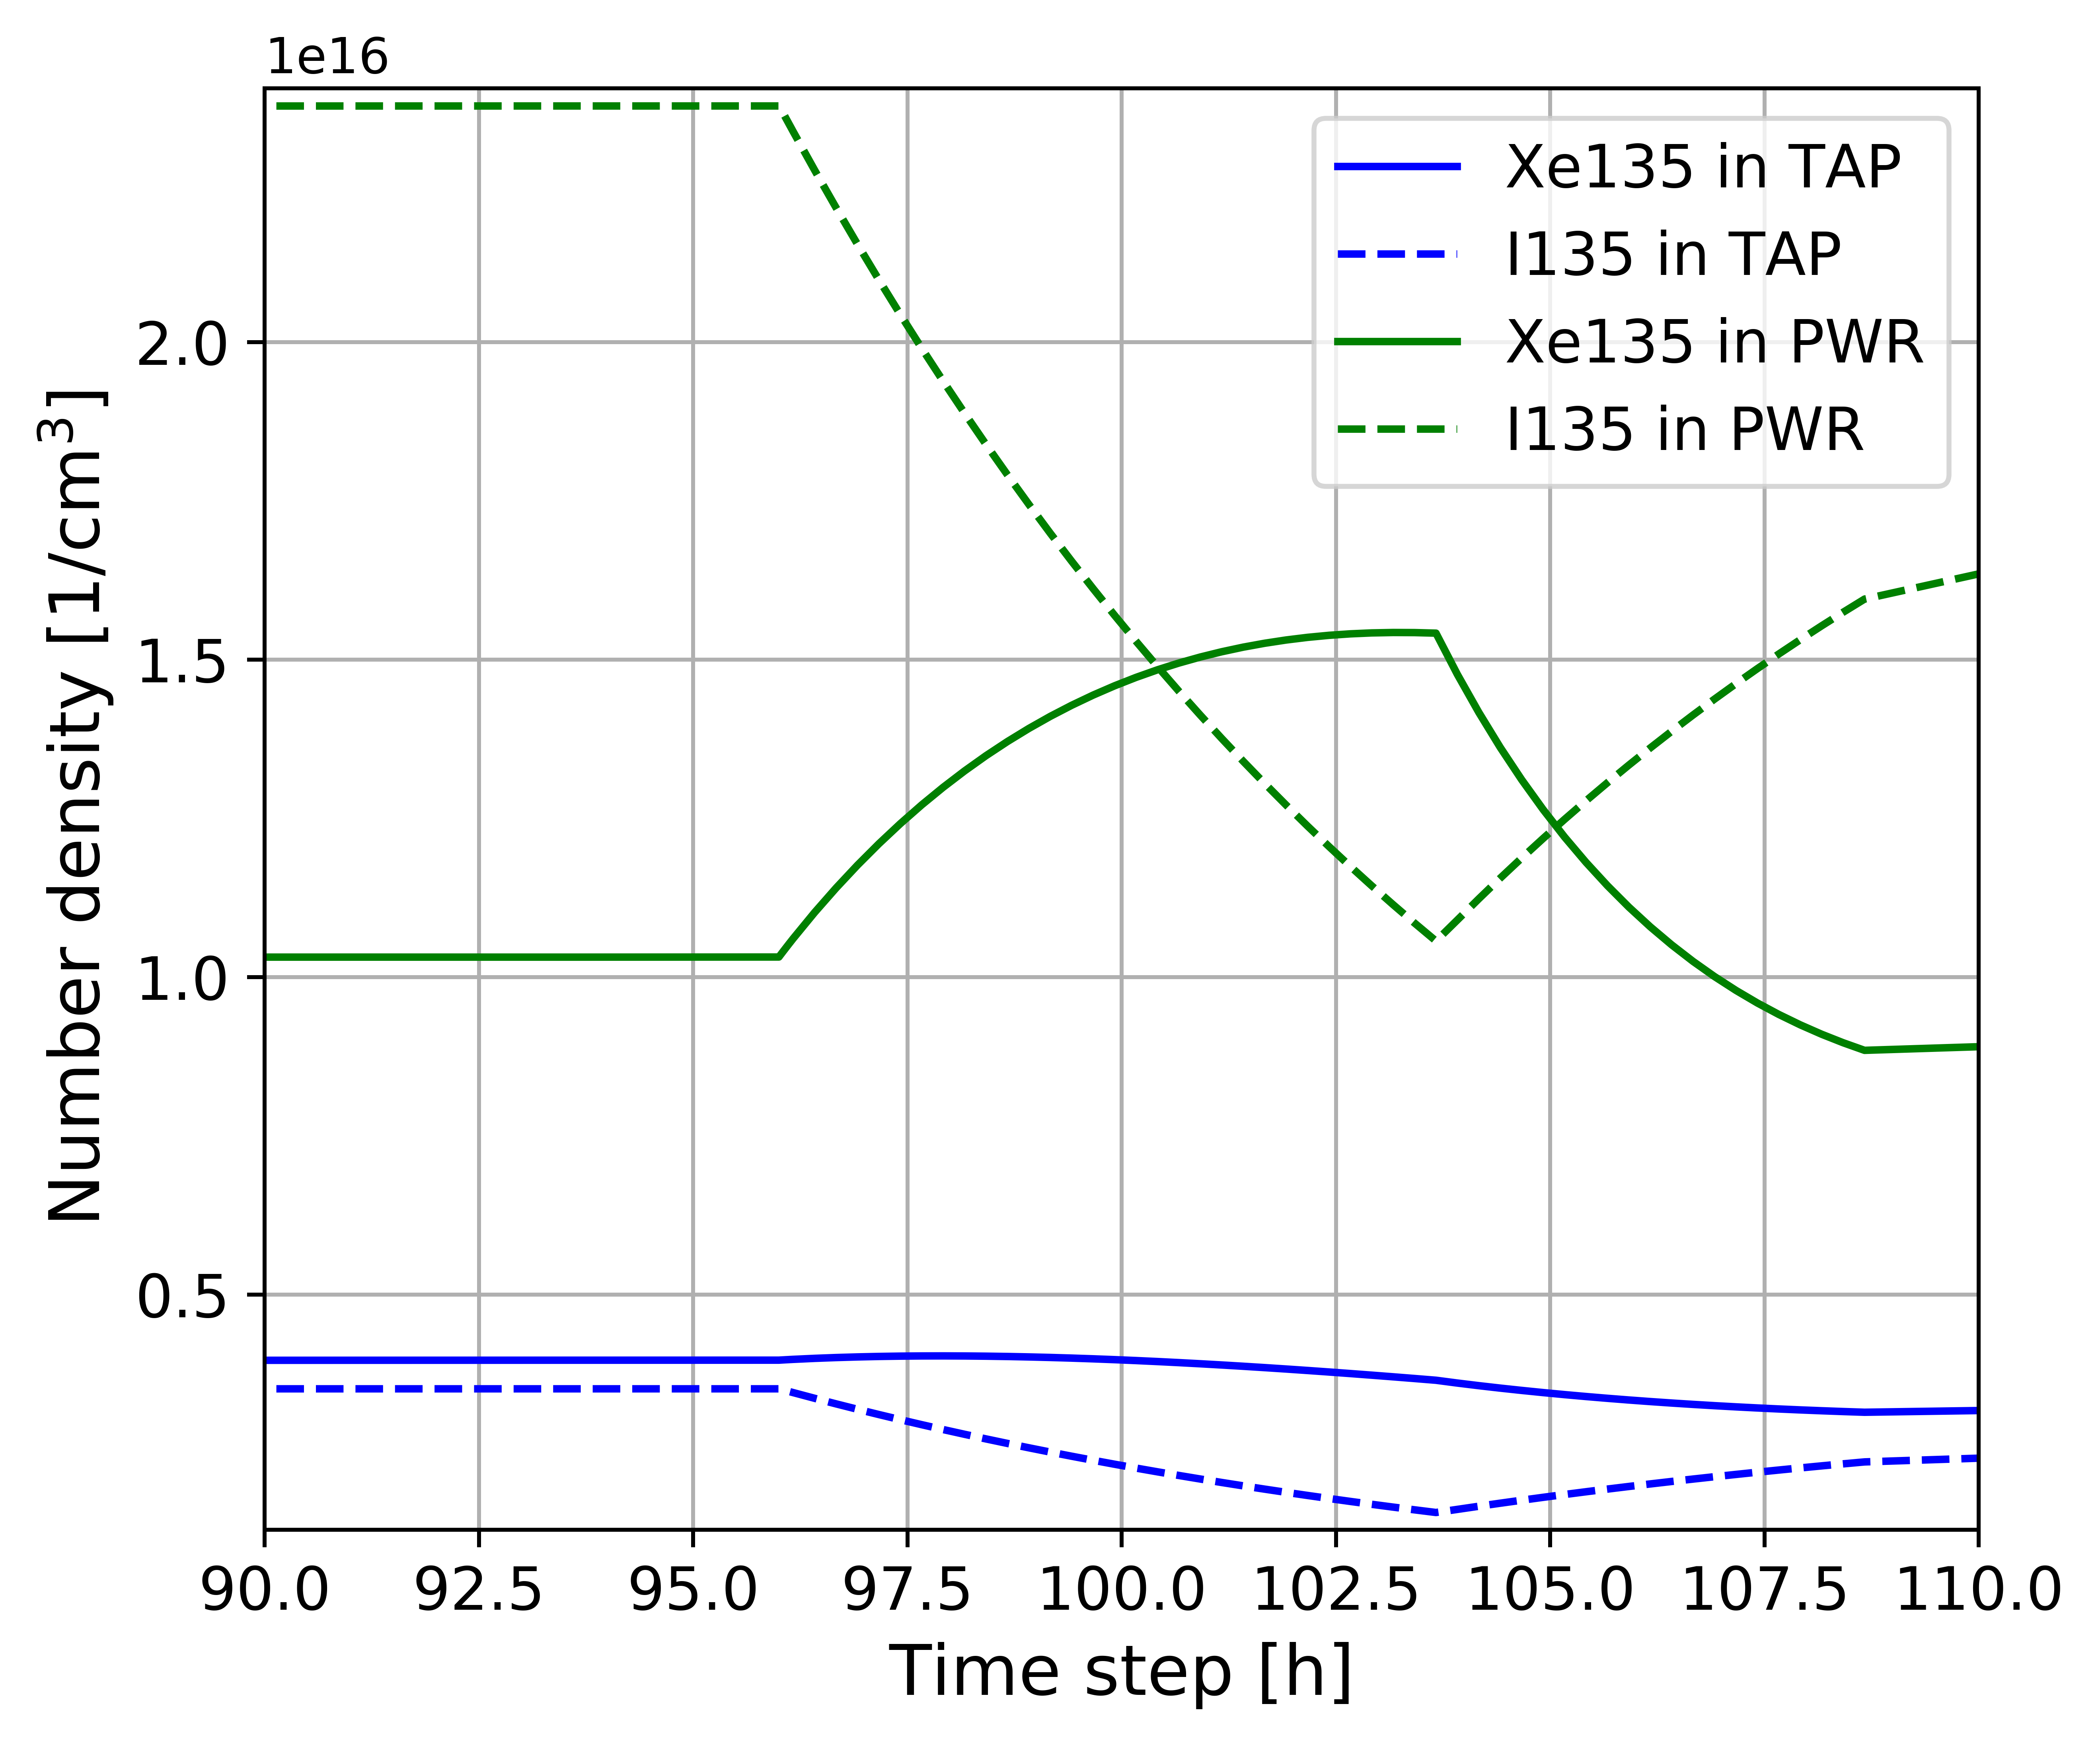
\includegraphics[width=\linewidth]{./images/tap_vs_pwr_xe_i_density.png}
		\caption{Atomic density of $^{135}$Xe and its main precursor 
		($^{135}$I) after shutdown.}
		\end{figure}
		\column{.5\textwidth}
			\vspace{+5mm}
		\begin{block}{Why no poisoning effect?}
			\begin{enumerate}             
				\item $^{135}$I/$^{135}$Xe number density ratio is 2.3 (PWR) 
				and 0.9 (TAP)
				\item $^{135}$I half-life 6.6h $<$ $^{135}$Xe half-life 9.2h
				\item PWR accumulated significant $^{135}$I inventory which 
				caused large xenon concentration  peak ($150\%$)
				\item In TAP, $^{135}$Xe gain from $^{135}$I decay did
				not overcome $^{135}$Xe decay loss
				\item Maybe because the neutron spectrum is different?
			\end{enumerate}
		\end{block}
	\end{columns}
\end{textblock*}
\end{frame}

\subsection{Neutron spectra}

\begin{frame}
\frametitle{Neutron spectra of PWR vs TAP}
\begin{textblock*}{12.3cm}(0.2cm,2cm) % {block width} (coords)
	\begin{columns}[t,onlytextwidth]
		\column{.6\textwidth}
		\begin{figure}[t]
			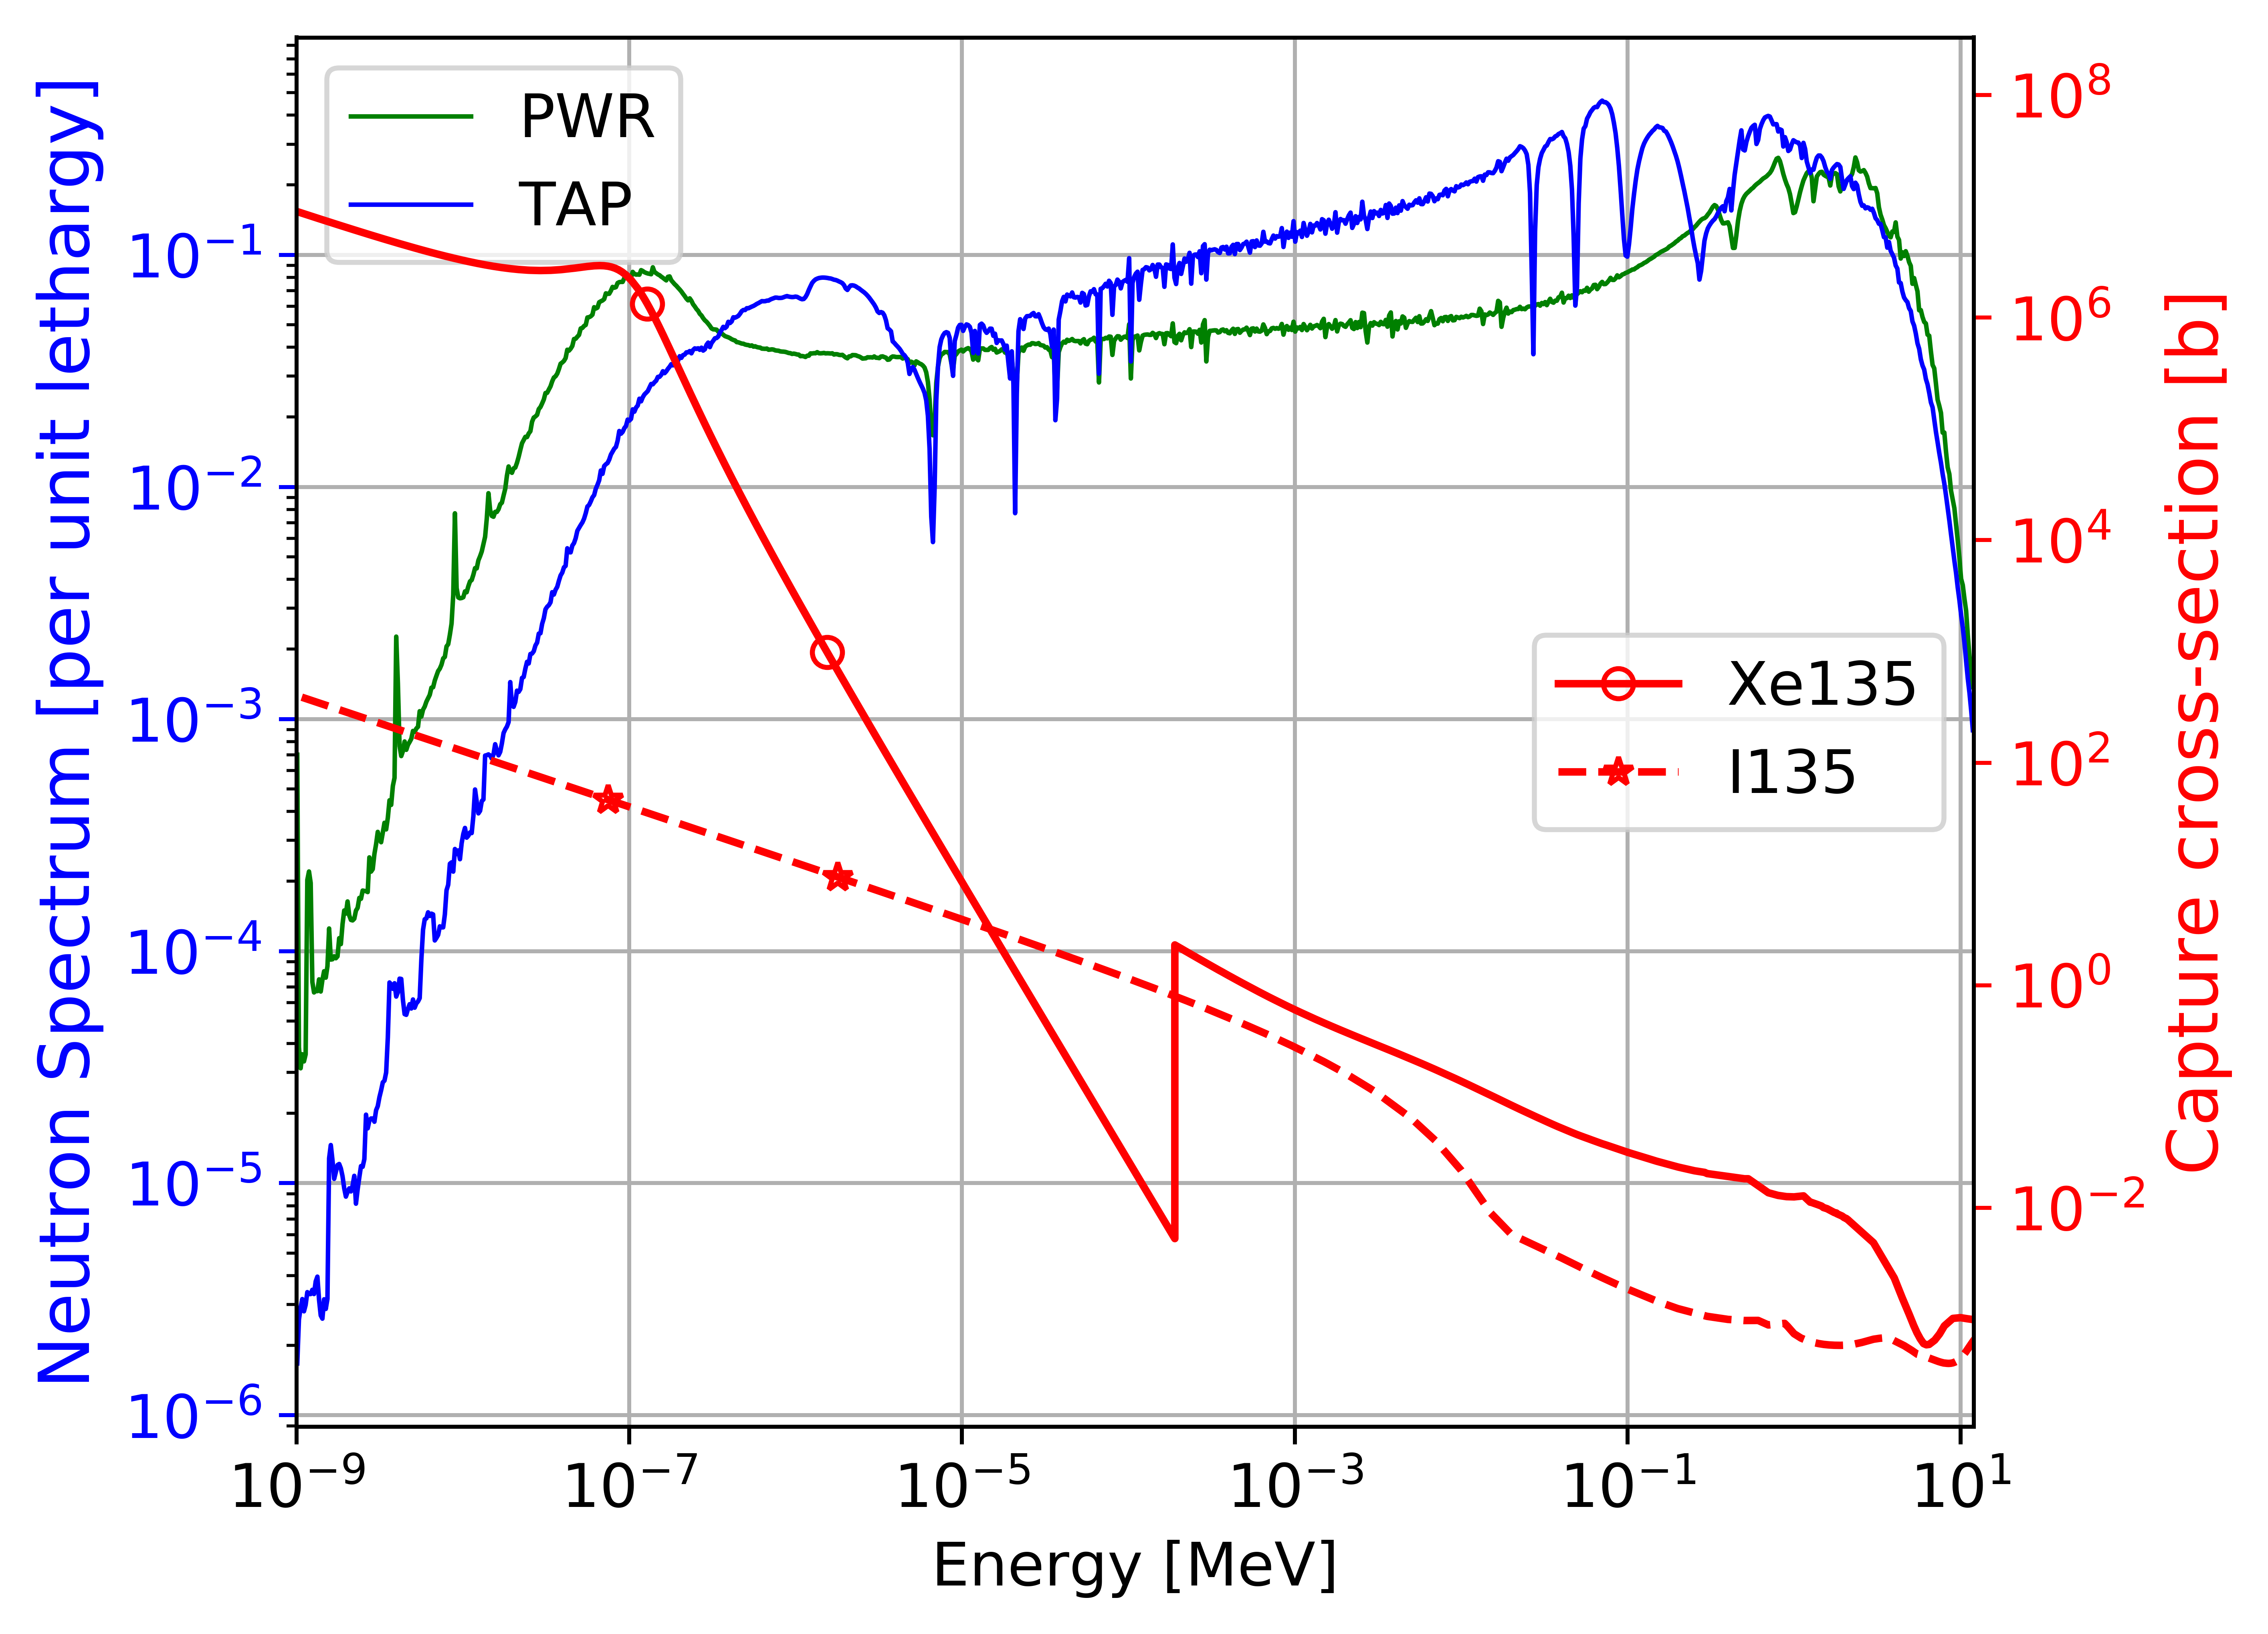
\includegraphics[width=\linewidth]{./images/spectra.png}
			\caption{Neutron spectra normalized by lethargy for the PWR and 
			TAP vs. $^{135}$Xe and $^{135}$I caption cross-section.}
		\end{figure}
	
	
		\column{.4\textwidth}
		\vspace{+1mm}
		\begin{block}{Why different $^{135}$I/$^{135}$Xe balance?}
			\begin{enumerate}             
				\item TAP at beginning-of-life has much harder spectrum than 
				PWR
				\item Harder neutron spectrum leads to weaker $^{135}$Xe 
				transmutation to $^{136}$Xe due to \textbf{strong energy 
				dependence of the capture cross-section}
				\item $\sigma_{(n,c)}$ slope is much steeper  for 
				$^{135}$Xe than for $^{135}$I
			\end{enumerate}
		\end{block}
	\end{columns}
\end{textblock*}
\end{frame}